\documentclass[aps,pra,amsmath,twocolumn,amssymb,superscriptaddress]{revtex4-1}
%=============================================================================
% BEGIN UNFORGIVABLE HACKS
%=============================================================================

\makeatletter
\def\@bibdataout@aps{%
 \immediate\write\@bibdataout{%
  @CONTROL{%
   apsrev41Control,author="08",editor="1",pages="0",title="0",year="1",eprint="1"%
  }%
 }%
 \if@filesw
  \immediate\write\@auxout{\string\citation{apsrev41Control}}%
 \fi
}%
\makeatother % Phew.

%=============================================================================
% END UNFORGIVABLE HACKS
%=============================================================================

\usepackage{amssymb}
\usepackage{amsthm}
\usepackage{amsfonts}
\usepackage{complexity}
\usepackage{graphicx}% Include figure files
\usepackage{dcolumn}% Align table columns on decimal point
\usepackage{bm}% bold math
\usepackage{hyperref}
\usepackage{enumerate}
\usepackage{algorithm}
\usepackage{algpseudocode}
    \renewcommand{\algorithmicrequire}{\textbf{Input:}}
    \renewcommand{\algorithmicensure}{\textbf{Output:}}
    \newcommand{\inlinecomment}[1]{\Comment {\footnotesize #1} \normalsize}
    \newcommand{\linecomment}[1]{\State \(\triangleright\) {\footnotesize #1} \normalsize}
    %\renewcommand{\algorithmiccomment}[1]{\State\(\triangleright\) #1}
    
\usepackage{multirow}

\newtheorem{theorem}{Theorem}
\newtheorem{lemma}{Lemma}
\newtheorem{definition}{Definition}
\newtheorem{corollary}{Corollary}

%    Q-circuit version 2
%    Copyright (C) 2004  Steve Flammia & Bryan Eastin
%    Last modified on: 9/16/2011
%
%    This program is free software; you can redistribute it and/or modify
%    it under the terms of the GNU General Public License as published by
%    the Free Software Foundation; either version 2 of the License, or
%    (at your option) any later version.
%
%    This program is distributed in the hope that it will be useful,
%    but WITHOUT ANY WARRANTY; without even the implied warranty of
%    MERCHANTABILITY or FITNESS FOR A PARTICULAR PURPOSE.  See the
%    GNU General Public License for more details.
%
%    You should have received a copy of the GNU General Public License
%    along with this program; if not, write to the Free Software
%    Foundation, Inc., 59 Temple Place, Suite 330, Boston, MA  02111-1307  USA

% Thanks to the Xy-pic guys, Kristoffer H Rose, Ross Moore, and Daniel Müllner,
% for their help in making Qcircuit work with Xy-pic version 3.8.  
% Thanks also to Dave Clader, Andrew Childs, Rafael Possignolo, Tyson Williams,
% Sergio Boixo, Cris Moore, Jonas Anderson, and Stephan Mertens for helping us test 
% and/or develop the new version.

\usepackage[color]{xy}
\UseCrayolaColors
\xyoption{matrix}
\xyoption{frame}
\xyoption{arrow}
\xyoption{arc}

\usepackage{ifpdf}
\ifpdf
\else
\PackageWarningNoLine{Qcircuit}{Qcircuit is loading in Postscript mode.  The Xy-pic options ps and dvips will be loaded.  If you wish to use other Postscript drivers for Xy-pic, you must modify the code in Qcircuit.tex}
%    The following options load the drivers most commonly required to
%    get proper Postscript output from Xy-pic.  Should these fail to work,
%    try replacing the following two lines with some of the other options
%    given in the Xy-pic reference manual.
\xyoption{ps}
\xyoption{dvips}
\fi

% The following resets Xy-pic matrix alignment to the pre-3.8 default, as
% required by Qcircuit.
\entrymodifiers={!C\entrybox}

%\newcommand{\bra}[1]{{\left\langle{#1}\right\vert}}
%\newcommand{\ket}[1]{{\left\vert{#1}\right\rangle}}
    % Defines Dirac notation. %7/5/07 added extra braces so that the commands will work in subscripts.
\newcommand{\qw}[1][-1]{\ar @{-} [0,#1]}
\newcommand{\eqw}[1][-1]{\ar @{-} @[Red] [0,#1]}
    % Defines a wire that connects horizontally.  By default it connects to the object on the left of the current object.
    % WARNING: Wire commands must appear after the gate in any given entry.
\newcommand{\qwx}[1][-1]{\ar @{-} [#1,0]}
    % Defines a wire that connects vertically.  By default it connects to the object above the current object.
    % WARNING: Wire commands must appear after the gate in any given entry.
\newcommand{\cw}[1][-1]{\ar @{=} [0,#1]}
    % Defines a classical wire that connects horizontally.  By default it connects to the object on the left of the current object.
    % WARNING: Wire commands must appear after the gate in any given entry.
\newcommand{\cwx}[1][-1]{\ar @{=} [#1,0]}
    % Defines a classical wire that connects vertically.  By default it connects to the object above the current object.
    % WARNING: Wire commands must appear after the gate in any given entry.
\newcommand{\gate}[1]{*+<.6em>{#1} \POS ="i","i"+UR;"i"+UL **\dir{-};"i"+DL **\dir{-};"i"+DR **\dir{-};"i"+UR **\dir{-},"i" \qw}
\newcommand{\eboxgate} [1]{*+<.6em>{#1} \POS ="i","i"+UR;"i"+UL **[red]\dir{-};"i"+DL **[red]\dir{-};"i"+DR **[red]\dir{-};"i"+UR **[red]\dir{-},"i" \eqw}
\newcommand{\circgate}[1]{*+<0.6em>[o][F-]{#1} \eqw}
\newcommand{\ecircgate}[1]{*+<0.6em>[o][F-:red]{#1} \eqw}
\newcommand{\filtergt}[1]{\eboxgate{\scriptscriptstyle{#1}}}
\newcommand{\idealdec}{*+<1.2em>{\phantom{*}} \POS ="i","i"+UL;"i"+DL **[red]\dir{-};"i"+R **[red]\dir{-};"i"+UL **[red]\dir{-},"i" \eqw}

    % Boxes the argument, making a gate.
\newcommand{\meter}{*=<1.8em,1.4em>{\xy ="j","j"-<.778em,.322em>;{"j"+<.778em,-.322em> \ellipse ur,_{}},"j"-<0em,.4em>;p+<.5em,.9em> **\dir{-},"j"+<2.2em,2.2em>*{},"j"-<2.2em,2.2em>*{} \endxy} \POS ="i","i"+UR;"i"+UL **\dir{-};"i"+DL **\dir{-};"i"+DR **\dir{-};"i"+UR **\dir{-},"i" \qw}
    % Inserts a measurement meter.
    % In case you're wondering, the constants .778em and .322em specify
    % one quarter of a circle with radius 1.1em.
    % The points added at + and - <2.2em,2.2em> are there to strech the
    % canvas, ensuring that the size is unaffected by erratic spacing issues
    % with the arc.
\newcommand{\measure}[1]{*+[F-:<.9em>]{#1} \qw}
    % Inserts a measurement bubble with user defined text.
\newcommand{\measuretab}[1]{*{\xy*+<.6em>{#1}="e";"e"+UL;"e"+UR **\dir{-};"e"+DR **\dir{-};"e"+DL **\dir{-};"e"+LC-<.5em,0em> **\dir{-};"e"+UL **\dir{-} \endxy} \qw}
    % Inserts a measurement tab with user defined text.
\newcommand{\measureD}[1]{*{\xy*+=<0em,.1em>{#1}="e";"e"+UR+<0em,.25em>;"e"+UL+<-.5em,.25em> **\dir{-};"e"+DL+<-.5em,-.25em> **\dir{-};"e"+DR+<0em,-.25em> **\dir{-};{"e"+UR+<0em,.25em>\ellipse^{}};"e"+C:,+(0,1)*{} \endxy} \qw}
\newcommand{\emeasureD}[1]{*{\xy*+=<0em,.1em>{#1}="e";"e"+UR+<0em,.25em>;"e"+UL+<-.5em,.25em> **[red]\dir{-};"e"+DL+<-.5em,-.25em> **[red]\dir{-};"e"+DR+<0em,-.25em> **[red]\dir{-};{"e"+UR+<0em,.25em>\ellipse{}};"e"+C:,+(0,1)*{} \endxy} \qw}
    % Inserts a D-shaped measurement gate with user defined text.
\newcommand{\multimeasure}[2]{*+<1em,.9em>{\hphantom{#2}} \qw \POS[0,0].[#1,0];p !C *{#2},p \drop\frm<.9em>{-}}
    % Draws a multiple qubit measurement bubble starting at the current position and spanning #1 additional gates below.
    % #2 gives the label for the gate.
    % You must use an argument of the same width as #2 in \ghost for the wires to connect properly on the lower lines.
\newcommand{\multimeasureD}[2]{*+<1em,.9em>{\hphantom{#2}} \POS [0,0]="i",[0,0].[#1,0]="e",!C *{#2},"e"+UR-<.8em,0em>;"e"+UL **\dir{-};"e"+DL **\dir{-};"e"+DR+<-.8em,0em> **\dir{-};{"e"+DR+<0em,.8em>\ellipse^{}};"e"+UR+<0em,-.8em> **\dir{-};{"e"+UR-<.8em,0em>\ellipse^{}},"i" \qw}
    % Draws a multiple qubit D-shaped measurement gate starting at the current position and spanning #1 additional gates below.
    % #2 gives the label for the gate.
    % You must use an argument of the same width as #2 in \ghost for the wires to connect properly on the lower lines.
\newcommand{\control}{*!<0em,.025em>-=-<.2em>{\bullet}}
    % Inserts an unconnected control.
\newcommand{\controlo}{*+<.01em>{\xy -<.095em>*\xycircle<.19em>{} \endxy}}
    % Inserts a unconnected control-on-0.
\newcommand{\ctrl}[1]{\control \qwx[#1] \qw}
    % Inserts a control and connects it to the object #1 wires below.
\newcommand{\ctrlo}[1]{\controlo \qwx[#1] \qw}
    % Inserts a control-on-0 and connects it to the object #1 wires below.
\newcommand{\targ}{*+<.02em,.02em>{\xy ="i","i"-<.39em,0em>;"i"+<.39em,0em> **\dir{-}, "i"-<0em,.39em>;"i"+<0em,.39em> **\dir{-},"i"*\xycircle<.4em>{} \endxy} \qw}
    % Inserts a CNOT target.
\newcommand{\qswap}{*=<0em>{\times} \qw}
    % Inserts half a swap gate.
    % Must be connected to the other swap with \qwx.
\newcommand{\multigate}[2]{*+<1em,.9em>{\hphantom{#2}} \POS [0,0]="i",[0,0].[#1,0]="e",!C *{#2},"e"+UR;"e"+UL **\dir{-};"e"+DL **\dir{-};"e"+DR **\dir{-};"e"+UR **\dir{-},"i" \qw}
    % Draws a multiple qubit gate starting at the current position and spanning #1 additional gates below.
    % #2 gives the label for the gate.
    % You must use an argument of the same width as #2 in \ghost for the wires to connect properly on the lower lines.
\newcommand{\ghost}[1]{*+<1em,.9em>{\hphantom{#1}} \qw}
    % Leaves space for \multigate on wires other than the one on which \multigate appears.  Without this command wires will cross your gate.
    % #1 should match the second argument in the corresponding \multigate.
\newcommand{\push}[1]{*{#1}}
    % Inserts #1, overriding the default that causes entries to have zero size.  This command takes the place of a gate.
    % Like a gate, it must precede any wire commands.
    % \push is useful for forcing columns apart.
    % NOTE: It might be useful to know that a gate is about 1.3 times the height of its contents.  I.e. \gate{M} is 1.3em tall.
    % WARNING: \push must appear before any wire commands and may not appear in an entry with a gate or label.
\newcommand{\gategroup}[6]{\POS"#1,#2"."#3,#2"."#1,#4"."#3,#4"!C*+<#5>\frm{#6}}
    % Constructs a box or bracket enclosing the square block spanning rows #1-#3 and columns=#2-#4.
    % The block is given a margin #5/2, so #5 should be a valid length.
    % #6 can take the following arguments -- or . or _\} or ^\} or \{ or \} or _) or ^) or ( or ) where the first two options yield dashed and
    % dotted boxes respectively, and the last eight options yield bottom, top, left, and right braces of the curly or normal variety.  See the Xy-pic reference manual for more options.
    % \gategroup can appear at the end of any gate entry, but it's good form to pick either the last entry or one of the corner gates.
    % BUG: \gategroup uses the four corner gates to determine the size of the bounding box.  Other gates may stick out of that box.  See \prop.

\newcommand{\rstick}[1]{*!L!<-.5em,0em>=<0em>{#1}}
    % Centers the left side of #1 in the cell.  Intended for lining up wire labels.  Note that non-gates have default size zero.
\newcommand{\lstick}[1]{*!R!<.5em,0em>=<0em>{#1}}
    % Centers the right side of #1 in the cell.  Intended for lining up wire labels.  Note that non-gates have default size zero.
\newcommand{\ustick}[1]{*!D!<0em,-.5em>=<0em>{#1}}
    % Centers the bottom of #1 in the cell.  Intended for lining up wire labels.  Note that non-gates have default size zero.
\newcommand{\dstick}[1]{*!U!<0em,.5em>=<0em>{#1}}
    % Centers the top of #1 in the cell.  Intended for lining up wire labels.  Note that non-gates have default size zero.
\newcommand{\Qcircuit}{\xymatrix @*=<0em>}
    % Defines \Qcircuit as an \xymatrix with entries of default size 0em.
\newcommand{\link}[2]{\ar @{-} [#1,#2]}
    % Draws a wire or connecting line to the element #1 rows down and #2 columns forward.
\newcommand{\pureghost}[1]{*+<1em,.9em>{\hphantom{#1}}}
    % Same as \ghost except it omits the wire leading to the left. 
%%%%%%%%%%%%%%%%%%%%%%%%%%%%%%%%%%%%%%%%%%%%%%%%%%%%%%%%%%%%%%%%%%%%%%%%%%%%%%%%%%%%%%%%%%
\newcommand{\multiprepareC}[2]{*+<1em,.9em>{\hphantom{#2}}\save[0,0].[#1,0];p\save !C
  *{#2},p+RU+<0em,0em>;+LU+<+.8em,0em> **\dir{-}\restore\save +RD;+RU **\dir{-}\restore\save
  +RD;+LD+<.8em,0em> **\dir{-} \restore\save +LD+<0em,.8em>;+LU-<0em,.8em> **\dir{-} \restore \POS
  !UL*!UL{\cir<.9em>{u_r}};!DL*!DL{\cir<.9em>{l_u}}\restore}
   % Draws a multiple qubit reverse-D-shaped preparation gate starting at the current position and spanning #1 additional gates below.
   % #2 gives the label for the gate.
   % You must use an argument of the same width as #2 in \pureghost for the wires to connect properly on
% the lower lines.
\newcommand{\prepareC}[1]{*{\xy*+=+<.5em>{\vphantom{#1\rule{0em}{.1em}}}*\cir{l^r};p\save*!L{#1} \restore\save+UC;+UC+<.5em,0em>*!L{\hphantom{#1}}+R **\dir{-} \restore\save+DC;+DC+<.5em,0em>*!L{\hphantom{#1}}+R **\dir{-} \restore\POS+UC+<.5em,0em>*!L{\hphantom{#1}}+R;+DC+<.5em,0em>*!L{\hphantom{#1}}+R **\dir{-} \endxy}}
   % Inserts a reverse-D-shaped preparation gate with user defined text.
\newcommand{\poloFantasmaCn}[1]{{{}^{#1}_{\phantom{#1}}}}



\def\ket#1{\left|#1\right\rangle}
\def\bra#1{\langle#1|}
\newcommand{\ketbra}[2]{|#1\rangle\!\langle#2|}
\newcommand{\braket}[2]{\langle#1|#2\rangle}
% \newcommand{\note}[1]{({\bf note: #1})}
\newcommand{\prob}[1]{{\rm Pr}\left(#1 \right)}
% \newcommand{\Tr}[1]{{\rm Tr}\!\left[#1 \right]}
\newcommand{\expect}[2]{{\mathbb{E}_{#2}}\!\left\{#1 \right\}}
\newcommand{\var}[2]{{\mathbb{V}_{#2}}\!\left\{#1 \right\}}
\newcommand{\CRej}{\text{RejF }}

\newcommand{\sinc}{\operatorname{sinc}}
\newcommand{\reset}{\mathrm{reset}}


% fix: supported only for revtex
%\newcommand{\openone}{\mathbb{I}}
% fix: unsupported with iopart
%\newcommand{\eqref}[1]{(\ref{#1})}

\newcommand{\sde}{\mathrm{sde}}
\newcommand{\Z}{\mathbb{Z}}
\newcommand{\RR}{\mathbb{R}}
\newcommand{\w}{\omega}
\newcommand{\Kap}{\kappa}

\newcommand{\Tchar}{$T$}
\newcommand{\T}{\Tchar~}
\newcommand{\TT}{\mathrm{T}}
\newcommand{\ClT}{\{{\rm Clifford}, \Tchar\}~}
\newcommand{\Tcount}{\Tchar--count~}
\newcommand{\Tcountper}{\Tchar--count}
\newcommand{\Tcounts}{\Tchar--counts~}
\newcommand{\Tdepth}{\Tchar--depth~}
\newcommand{\Zr}{\Z[i,1/\sqrt{2}]}
\newcommand{\ve}{\varepsilon}

\newcommand{\eq}[1]{\hyperref[eq:#1]{(\ref*{eq:#1})}}
\renewcommand{\sec}[1]{\hyperref[sec:#1]{Section~\ref*{sec:#1}}}
%\newcommand{\app}[1]{\hyperref[app:#1]{Appendix~\ref*{app:#1}}}
\newcommand{\app}[1]{the supplentary material}
\newcommand{\fig}[1]{\hyperref[fig:#1]{Figure~\ref*{fig:#1}}}
\newcommand{\thm}[1]{\hyperref[thm:#1]{Theorem~\ref*{thm:#1}}}
\newcommand{\lem}[1]{\hyperref[lem:#1]{Lemma~\ref*{lem:#1}}}
\newcommand{\tab}[1]{\hyperref[tab:#1]{Table~\ref*{tab:#1}}}
\newcommand{\cor}[1]{\hyperref[cor:#1]{Corollary~\ref*{cor:#1}}}
\newcommand{\alg}[1]{\hyperref[alg:#1]{Algorithm~\ref*{alg:#1}}}
\newcommand{\defn}[1]{\hyperref[def:#1]{Definition~\ref*{def:#1}}}


\newcommand{\targfix}{\qw {\xy {<0em,0em> \ar @{ - } +<.39em,0em>
\ar @{ - } -<.39em,0em> \ar @{ - } +
<0em,.39em> \ar @{ - }
-<0em,.39em>},<0em,0em>*{\rule{.01em}{.01em}}*+<.8em>\frm{o}
\endxy}}

\newenvironment{proofof}[1]{\begin{trivlist}\item[]{\flushleft\it
Proof of~#1.}}
{\qed\end{trivlist}}


\newcommand{\cu}[1]{{\textcolor{red}{#1}}}
\newcommand{\tout}[1]{{}}
% \newcommand{\beq}{\begin{equation}}
% \newcommand{\eeq}{\end{equation}}
% \newcommand{\beqa}{\begin{eqnarray}}
\newcommand{\good}{{\rm good}}
\newcommand{\bad}{{\rm bad}}
% \newcommand{\eeqa}{\end{eqnarray}}

\newcommand{\id}{\openone}
%\newcommand{\id}{\mathbb{I}}

\newcommand{\etal}{\emph{et al.}}
\newcommand{\ii}{\mathrm{i}}
\newcommand{\ee}{\mathrm{e}}

\hyphenation{FPGA}
\hyphenation{FPGAs}
\hyphenation{RFPE}

%%%%%%%%%%%%%%%%%%%%%%% a bit nicer hypelinks %%%%%%%%%%%%%%%%%%%%%%%%%%%%%

\usepackage[usenames,dvipsnames]{xcolor}
\hypersetup{
    colorlinks=true,       % false: boxed links; true: colored links
    linkcolor=Maroon,          % color of internal links (change box color with linkbordercolor)
    citecolor=OliveGreen,        % color of links to bibliography
    filecolor=magenta,      % color of file links
    urlcolor=Blue           % color of external links
}

%%%%%%%%%%%%%%%%%%%%%%% a bit nicer hypelinks %%%%%%%%%%%%%%%%%%%%%%%%%%%%%

\begin{document}

%=============================================================================
% FRONT MATTER
%=============================================================================

\title{Efficient Bayesian Phase Estimation}
\author{Nathan Wiebe}
\affiliation{Quantum Architectures and Computation Group, Microsoft Research, Redmond, WA (USA)}

\author{Chris Granade}
\affiliation{Centre for Engineered Quantum Systems, Sydney, NSW (Australia)}
\affiliation{School of Physics, University of Sydney, Sydney, NSW (Australia)}

\begin{abstract}
We introduce a new method called rejection filtering that we use to perform adaptive Bayesian phase estimation.  Our approach has several advantages: it is classically efficient, easy to implement, achieves Heisenberg limited scaling, resists depolarizing noise, tracks time dependent eigenstates, recovers from failures and can be run on an FPGA.  It also outperforms existing methods such as Kitaev's method and information theory phase estimation.
\end{abstract}

\maketitle

%=============================================================================
\section{Introduction}
\label{sec:intro}
%=============================================================================

Eigenvalue estimation has been a cornerstone of physics since the dawn of spectroscopy.  In recent years, ideas from quantum information have revolutionized the ways that we estimate these values by providing methods that require exponentially fewer experiments than statistical sampling and total experimental time that saturates the Heisenberg limit~\cite{Kit96,berry_optimal_2000,kitaev2002classical,higgins2007entanglement,BHB+09,GTA+06,hentschel_machine_2010,SHF14}, which is the best possible scaling allowed by quantum mechanics.  This quantum approach, known as phase estimation, is crucial to acheive many of the celebrated speedups promised by quantum computing~\cite{shor_polynomial-time_1995,BHM+02,ADL+05,harrow2009quantum,lanyon2010towards}.

While great progress has been made towards optimizing phase estimation, a number of gaps remain.  Most notably, existing approaches either require a large number of ancilla qubits, are classically inefficient or fail to extract information about the phase as efficiently as their classically inefficient brethren.  Moreover, the majority of these methods are not analyzed in the presence of noise or other experimental imperfections.  Finally, these approaches typically assume that the phase is static, or quasi-static, throughout the experiment.  This precludes phase estimation from tracking time dependent drifts in phase.  These gaps mean that many phase estimation algorithms are not known to be robust enough to be used in many modern day experiments.

%The need for efficient phase estimation algorithms is especially poignant for Shor's algorithm~\cite{shor_polynomial-time_1995}, wherein the unknown eigenphases must be estimated to hundreds of bits of precision.  In order
%for the algorithm to be practical for this application, the phase estimation algorithm must only use a logarithmic number of measurements and the classical processing used to infer the phase must also be efficient.
%This excludes many existing iterative phase estimation methods that achieve logarithmic scaling.  Other methods are both classically and quantumly efficient~\cite{Kit96,kitaev2002classical,higgins2007entanglement,BHB+09,SHF14}, but often fail to extract information about the phase as efficiently as their classically inefficient brethren or require many ancilla qubits.

Here we address these shortcomings by proposing an approach to iterative phase estimation that is based on a new inference method that we call \emph{rejection filtering}, and by providing an efficient heuristic for adaptively selecting near-optimal experiments. We call the phase estimation algorithm that follows from rejection filtering phase estimation or \emph{RFPE}.  Our algorithm numerically approximates Bayesian inference on the measurement outcomes to estimate the most likely phase and its uncertainty.  Unlike the numerical methods for Bayesian inference studied in~\cite{granade_robust_2012, stenberg_efficient_2014}, the method has miniscule memory requirements which permits it to be employed in a memory limited environment like a field programmable gate array (FPGA).  Our algorithm also inherits from Bayesian inference the ability follow drifting eigenphases without needing to explicitly model the dynamics of the phase.  Finally, we propose a novel method for detecting and correcting inference errors that allows the method to track a state's depolarization in real time.  These new capabilities constitute an important advance for the field and underscore the relevance of approximate Bayesian inference to physics.
%
%RFPE is classically efficient, requires a logarithmic number of operations, saturates the Heisenberg bound, 
%is robust to experimental imperfections such as depolarizing noise  and
%small systematic errors, reports the uncertainty in the estimate of the phase, can track time-dependent phases and can be employed in a memory limited environment like in an field programmable gate array (FPGA).

Before going into detail about our algorithm we will first review the iterative phase estimation circuit and Bayesian approaches to phase estimation.  
Iterative phase estimation learns the eigenvalue of a given eigenvector of a unitary matrix
$U\in \mathbb{C}^{2^n \times 2^n}$ from a set of experiments that are performed on the quantum circuit~\cite{NC00}
\begin{equation*}
    \Qcircuit @C=1em @R=1em {
        \lstick{\ket{0}}    & \gate{H}  & \gate{Z(-M \theta)}   & \ctrl{1}   & \gate{H} & \meter & \cw \\
        \lstick{\ket{\phi}} & {/} \qw   & \qw                   & \gate{U^M} & \qw      & \qw    & \qw
    }
\end{equation*}
where $H$ is the Hadamard gate, $U\ket{\phi} = \ee^{\ii\phi}\ket{\phi}$ for an unknown eigenphase $\phi \in \mathbb{R}$, $\ket{\phi}\in \mathbb{C}^{2^n}$, 
$M\in\mathbb{N}$ specifies how many applications of $U$ are applied conditioned on the ancilla qubit being $1$,
and where $Z(M \theta) = \ee^{\ii M \theta Z}$ for the Pauli operator $Z$ is a rotation that can be used to compare the eigenphase of $U$ to
a known reference value.  Most iterative phase estimation algorithms use this circuit to infer the bits
in a binary expansion of $\phi$.  The process can be made optimal (up to $\log^*$ factors~\cite{SHF14}) and
also classically efficient.



%Our work addresses these problems by not only providing a method for
%performing an efficient form of Bayesian phase estimation but also giving an
%expedient heuristic for adaptively choosing approximately optimal experiments.
%We illustrate this by showing that our algorithm not only exhibits the same
%Heisenberg limited scaling of phase estimation and
%continues to learn even when decoherence or other experimental imperfections prevent traditional phase estimation
%methods from working.

%=============================================================================
\section{Bayesian Phase Estimation}
\label{sec:bayesian-phase-est}
%=============================================================================

Bayesian phase estimation involves performing a 
set of experiments and then updating the prior distribution using Bayes' rule
\cite{berry_optimal_2000,berry_optimal_2001,SHF14}.
For example, if an experiment is performed with using $M$ repetitions of $U$,
$Z(M \theta)$ and a measurement outcome $E\in \{0,1\}$ is observed then Bayes'
rule states that the \emph{posterior probability} distribution for $\phi$
after observing the datum is
\begin{equation}
P(\phi|E;\theta,M) = \frac{P(E|\phi;\theta,M)P(\phi)}{\int P(E|\phi;\theta,M)P(\phi)\mathrm{d}{\phi}}.\label{eq:update}
\end{equation}
The likelihood
function for phase estimation, $P(0|\phi;\theta,M)$,  is
\begin{gather}
    \label{eq:likenodecohere}
    \begin{aligned}
        P(0|\phi;\theta,M) & = \frac{1+\cos(M[\phi +\theta])}{2},\\
        P(1|\phi;\theta,M) & = \frac{1-\cos(M[\phi +\theta])}{2}.
    \end{aligned}
\end{gather}
Note that we have assumed perfect visibility of measurements in this likelihood function;
that assumption can be readily relaxed \cite{ferrie_how_2013,cappellaro_spin_2012}, such that
we consider the perfect visibility case for clarity.
After using~\eq{update} to update the posterior distribution we then set the prior distribution to equal the posterior distribution.  This process is then repeated for each of the experiments in the data set.

Unlike conventional methods, Bayesian inference returns a posterior
distribution over the phase. The mean and standard deviation of this
distribution provide an estimate of the true eigenvalue and the algorithm's
uncertainty in that value. More sophisticated estimates of uncertainty, such
as credible regions, can also be extracted from the posterior
distribution~\cite{granade_robust_2012,ferrie_high_2014}.  

%These uncertainty estimates are crucial for the experiment design phase of  RFPE
% and also because they allow the protocol to be terminated when a threshold accuracy has been reached.

\begin{figure}[t!]
    \begin{centering}
        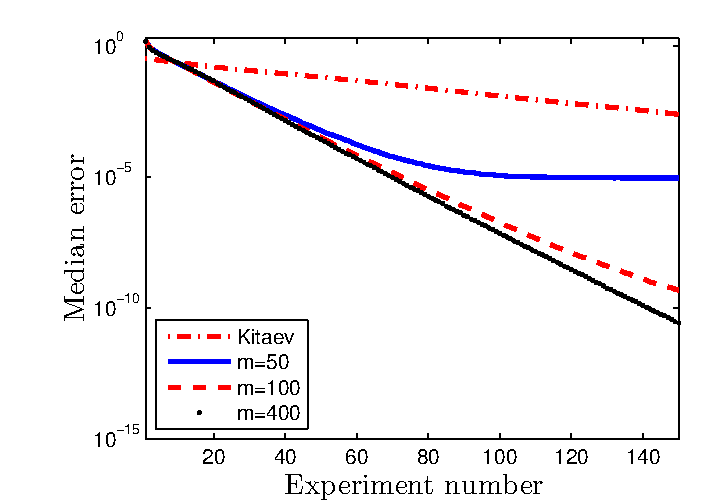
\includegraphics[width=0.8\linewidth]{PEerror.pdf}
    \end{centering}
    \caption{\label{fig:PEerror}
     Median errors in phase estimation for 10~000 random initial choices of the true eigenphase.
    }
\end{figure}





%=============================================================================
\section{Approximate Bayesian Phase Estimation}
%=============================================================================

Exact Bayesian inference is impossible if the eigenphases are
continuous so approximations are needed to
make the procedure tractable.  Rather than na\"ively discritizing the prior
distribution, modern methods discretize by sampling from the prior and
then perform Bayesian inference on the discrete set of samples (often called
``particles'').  These particle filter methods methods are quite powerful and
have become a mainstay in computer vision and machine
learning~\cite{haykin2004kalman,smith2013sequential,isard_condensationconditional_1998}.


Despite the power of these methods, they are hard to implement and even
harder to deploy in a memory limited environment such as on an embedded
controller or an FPGA. With the increasing use of FPGAs in the control of
quantum information experiments
\cite{shulman_suppressing_2014,casagrande_design_2014,hornibrook_cryogenic_2015},
overcoming this limitation presents a
significant advantage to modern experiment design. 

RFPE follows a much simpler approach. Rather than using a set of hypotheses that implicitly
define a model for the system, we posit a prior model and directly update it
to find a model for our posterior distribution.  We achieve this by using a
Gaussian with mean $\mu$ and variance $\sigma^2$ to model our initial prior, perform a Bayesian update on samples
drawn from the distribution and then refit the updated samples to a Gaussian.
This strategy is used in a number of particle filter methods such as the extended Kalman filter and assumed density
filtering~\cite{haykin2004kalman,opper1998bayesian}.  We further optimize
this process by approximating the Bayesian inference step using rejection
sampling.  This can reduce the memory required by a factor of $1~000$ or more,
as we need only consider a single sample at a time. Our algorithm is described
below and pseudocode is given in \app{pseudocode}.

\begin{figure}[t!]
    \begin{centering}
        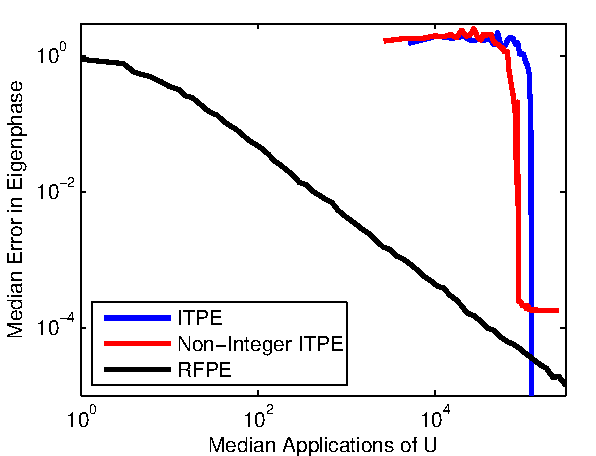
\includegraphics[width=0.723\linewidth]{ITPEcmp.pdf}
    \end{centering}
    \caption{\label{fig:ITPEcmp}
     Comparison of RFPE to ITPE for $t=10~000$ with $100$ samples for $\phi_{\rm true} = 2\pi k/t$ at each measurement.  
    }
\end{figure}







\begin{enumerate}
\item Perform experiment for given $\theta$, $M$ and observe outcome $E\in \{0,1\}$.
\item Draw $m$ samples from $\mathcal{N}(\phi|\mu,\sigma^2)$.
\item For each sample, $\phi_j$, assign $\phi_j$ to $\Phi_{\rm accept}$ with probability $P(E|\phi_j;\theta,M)/\kappa_E$, where $\kappa_E\in (0,1]$ is a constant s.t. $P(E|\phi_j;\theta,M)/\kappa_E\le 1$ for all $\phi_j,E$.
\item Return $\mu = \mathbb{E}(\Phi_{\rm accept})$ and $\sigma =\sqrt{\mathbb{V}(\Phi_{\rm accept})}$.
\end{enumerate}

The resultant samples are equivalent to those drawn from the posterior distribution
$P(\phi|E;M,\theta)$.  To see this, note that the probability density of a sample being accepted at $\phi=\phi_j$ is $ P(E | \phi; \theta, M) \mathcal{N}(\phi|\mu,\sigma^2)$.  Eqn~\eq{update} then implies 
\begin{equation}
    P(E | \phi; \theta, M) \mathcal{N}(\phi|\mu,\sigma^2) \propto P(\phi | E; \theta, M),
\end{equation}
which implies that the accepted samples are drawn from the posterior distribution.  

Although it is difficult to concretely predict the value of $m$ needed to make the error in the inference small, we show in \app{stability} that $m$ must scale at least as the inverse square of the relative fluctuations in the likelihood function.  Similarly, Markov's inequality shows that $m$ must scale at least as $\kappa_E/\int P(E|\phi;\theta,M)P(\phi) \mathrm{d}\phi$ to ensure that, with high probability, the mean can be accurately estimated from the accepted samples.  We introduce $\kappa_E$ to compensate for small expected likelihoods.

\begin{figure}[t!]
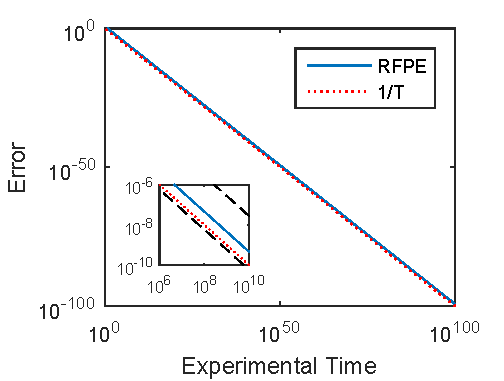
\includegraphics[width=0.9\linewidth]{Longpet2.pdf}
\caption{Median error vs evolution time for rejection filter phase estimation for the case where $M$ is continuous and $T=\sum_i M_i$.  The median error scales roughly as $4.7/T$, and the dashed lines in the inset figure give a $95\%$ confidence interval.}\label{fig:rms}
\end{figure}

The main issue that remains is how to optimally choose the parameters $\theta$
and $M$. One approach is to locally optimize the Bayes
risk~\cite{granade_robust_2012}, but the resulting calculation can be too
expensive to carry out in online experiments that provide experimental results
at a rate of tens of megahertz or faster.
This can be avoided using precomputed
measurement settings
\cite{sergeevich_characterization_2011}
or \emph{policies} \cite{hentschel_machine_2010,hayes_swarm_2014}, which
can substantially reduce the computational time needed to perform an online inference. These approaches,
however, \emph{a priori} limit the number of measurements to
be performed, and can require significant amounts of memory to store the policy.

Fortunately, the particle guess heuristic (PGH) can give
expedient and
near-optimal experiments for this class of likelihood
functions in an online fashion, and with no precomputation
required~\cite{wiebe_hamiltonian_2014},
\begin{align}
    M &= \left\lceil\frac{1.25}{\sigma}\right\rceil,~
    \theta \sim P(\phi).\label{eq:PGH}
\end{align}
The constant $1.25$ is chosen as it works well empirically.



\fig{PEerror} shows the error incurred using RFPE.  The most obvious feature is that the error shrinks exponentially with the number of experiments (which is proportional to the evolution time under the PGH) for $m>100$.  Roughly $150$ experiments are needed for the method to provide $32$ bits of accuracy in the median case.
We discuss the scaling in the mean in \app{var-reduction}.

The number of experiments needed by RFPE scales as $O(\log(1/\epsilon))$, where $\epsilon$ is the target uncertainty, rather than the $O(\log(1/\epsilon)\log\log(1/\epsilon))$ scaling of Kitaev's method~\cite{Kit96,kitaev2002classical}.  
 RFPE should therefore offer advantages for implementing Shor's algorithm in small quantum devices.
Concretely, after $150$ experiments the median error for Kitaev's algorithm (with $s=10$) is roughly $10^7$ times that of RFPE.  $O(\log(1/\epsilon))$ scaling  is further observed over $100$ orders of magnitude in $\epsilon$ in the appendix and is optimal (as seen from a simple counting argument).


%Although the number of experiments needed is small, the experimental time need
%not be.  If the error shrinks as $\epsilon\in \Theta(\ee^{-\lambda N})$ where
%$N$ is the experiment number then $T_{\exp}\in O(\sum_{N=1}^{N_{\max}} \ee^{\lambda N})\in O(\ee^{\lambda N_{\rm max}})\in O(1/\epsilon)$.  The
%time required saturates the Heisenberg limit, up to a multiplicative constant.
%Specifically, $\lambda\approx 0.17$ for RFPE.



\fig{ITPEcmp} compares RFPE to the information-theory phase estimation (ITPE) method of Svore~\etal~\cite{SHF14}.  Although ITPE is inefficient and is non--adaptive, it is exact and so it is a natural benchmark to compare RFPE against.  We find  ITPE requires nearly five times the applications of $U$ if $\phi=2\pi k/t$ for integer $k<t$ and $t=10~000$.

\begin{figure}[t!]
    \begin{centering}
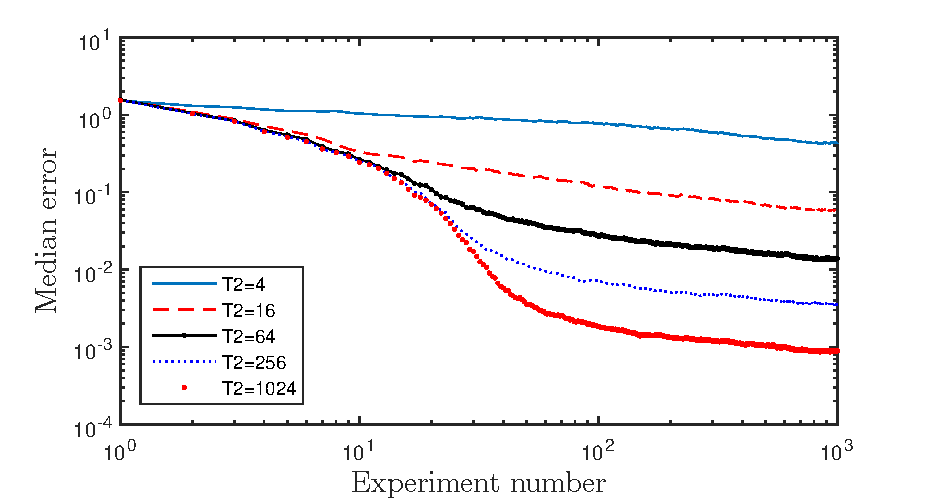
\includegraphics[width=0.95\linewidth]{T2plot_full.pdf}
%        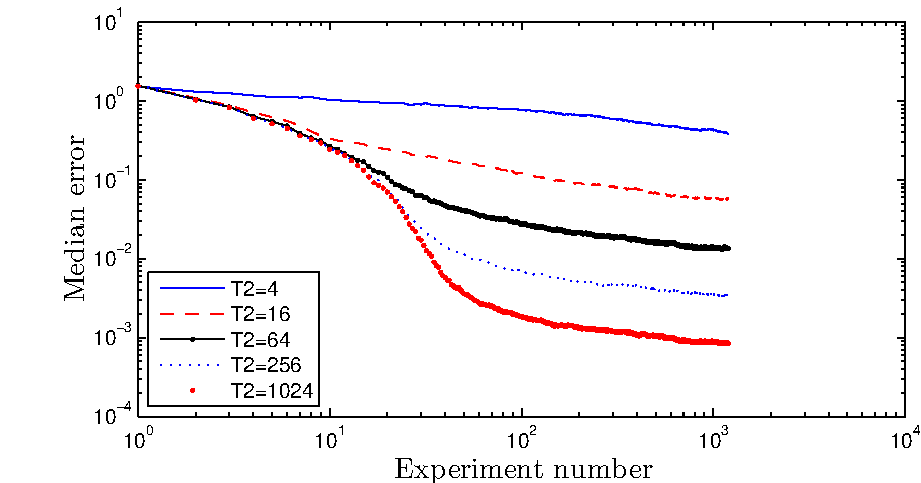
\includegraphics[width=0.45\linewidth]{T2plot.pdf}
    \end{centering}
    \caption{\label{fig:T2plot}
Median errors for phase estimation in decohering systems for experiments constrained to use $M\le T_2$.  We take $m=12~000$ and use $1~000$ random samples to generate the data above.  The initial state is taken to be a randomly chosen eigenstate in all cases.
    }
\end{figure}
Conversely,
ITPE requires only $25$ measurements to identify the phase with $50\%$
probability whereas RFPE requires $51$ experiments if $k$ is an integer.  If
the true value of $k$ is real-valued and ITPE is left unmodified, then  ITPE
fails to learn in the median because the long evolution times chosen lead to
contradictory possibilities that prevents ITPE from converging to a unique answer.  We correct
this by choosing $M\rightarrow \lceil M/2\rceil$ in such cases, which increases the number
of experiments to $35$ but also reduces the experimental time below that of
unmodified ITPE.  All three methods therefore
tradeoff experimental and computational resources differently.  This is especially salient because ITPE is inefficient unlike RFPE.

\begin{figure*}
    \begin{centering}
        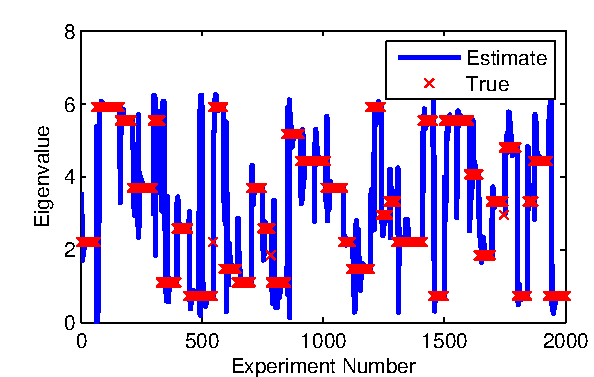
\includegraphics[width=0.4\linewidth]{Errtrack1.pdf}
        \hspace{5mm}
        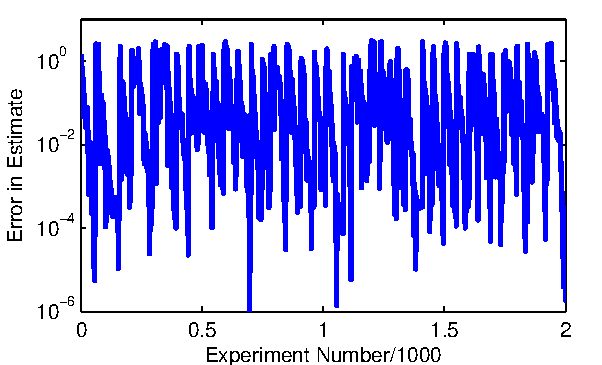
\includegraphics[width=0.4\linewidth]{Errtrack2.pdf}
    \end{centering}
    \caption{\label{fig:Errplot}
        Instantaneous estimate of the eigenphase  for a system with $16$ eigenvalues, $\Delta=0$, $\tau=0.1$ and $T_2=10^4$.
    }
\end{figure*}

In contrast to Shor's algorithm, in metrological and simulation applications the scaling of the error with the total number of applications of $U$ needed  (or in the case where $M$ is continuous, the total evolution time) is the most significant metric.
The Heisenberg bound states that the error optimally scales as $1/T=1/\sum_i M_i$ here.
\fig{rms} shows that this scaling is saturated for RFPE.  We further observe that the mean error, the
root-mean square error and a $95\%$ confidence interval for the error follow an optimal $O(1/T)$ scaling.
RFPE therefore saturates optimal scaling in this setting as well.


%\fig{rms} examines the performance of RFPE as a function of the total evolution number of applications of $U$ needed to achieve an error threshold.
%The data conforms to the $O(1/T)$ scaling expected from the Heisenberg bound.  Further details are given in the appendix.


\subsection{Phase estimation with depolarizing noise}
A criticism that has been levied lately at phase estimation methods is that they can be impractical to execute on non--fault tolerant quantum hardware~\cite{PMS+14,MBL+14,WHT15}.  This is because phase estimation attains its quadratic advantage over statistical sampling by using exponentially long evolutions.  Decoherence causes the resultant phases to become randomized as time progresses, ultimately resulting in
$\lim_{M\rightarrow \infty} P(0|\phi;\theta,M) = \frac{1}{2}$.
Measurements convey no information in this limit.  It similarly may be tempting to think that decoherence fundamentally limits the accuracy of phase estimation.   Bayesian inference to can, however, estimate $\phi$ using experiments with $M \approx T_2$~\cite{granade_robust_2012} for some noise models.  

We model the effect of decoherence on the system by assuming the existence of a \emph{decoherence time} $T_2$ such that
\begin{gather}
    \label{eq:likedecohere}
    \begin{aligned}
        P(0|\phi) & = \ee^{-M/T_2}\left(\frac{1+\cos(M[\phi -\theta])}{2}\right)+\frac{1-\ee^{-M/T_2}}{2},\\
        P(1|\phi) & = \ee^{-M/T_2}\left(\frac{1-\cos(M[\phi -\theta])}{2}\right)+\frac{1-\ee^{-M/T_2}}{2}.
    \end{aligned}
\end{gather}
This model is appropriate when a controlled $U$ gate is slow relative to the $H$ and $Z$-rotation gates, as is appropriate in quantum simulation.  %We assume in the following that $T_2$ is known. 
 

Since $T_2$ places a limitation on our ability to learn, we propose a variation to \eq{PGH},
\begin{equation}
    \label{eq:pgh2}
    M = \min\left\{\left\lceil\frac{1.25}{\sigma}\right\rceil, T_2 \right\}.
\end{equation}
The experiments yielded by~\eq{pgh2} resemble locally optimized experiments for frequency estimation, which saturate the Cram\'er-Rao bound \cite{ferrie_how_2013}; however,~\eq{pgh2} requires nearly 100 fold less computing time to select an experiment.
The choice to cut off $M$ at $T_2$ can be understood using the following argument.  The Cram\'er-Rao bound for frequency estimation scales as $O(M^{-2})$~\cite{WGC15} in the absence of decoherence.  Eqn.~\eq{likedecohere} suggests that decoherence causes the posterior variance to increase as $O(\exp(2M/T_2))$. { Calculus reveals that $M=T_2$ optimally trades off these tendencies~\cite{ferrie_how_2013}, which justifies~\eq{pgh2}.

\fig{T2plot} shows that RFPE smoothly transitions between the exponential scaling expected at short times and the polynomial scaling expected when decoherence becomes significant.  The error scales roughly as $1/N^{0.6}$ in this polynomial regime, which is comparable to the $1/\sqrt{N}$ scaling expected from statistical sampling.  Depolarizing noise, or diminished visibility~\cite{hayes_swarm_2014}, therefore does not \emph{necessarily} limit the accuracy of phase estimation.



%=============================================================================
\section{Tracking Eigenphases}
%=============================================================================

\fig{T2plot} shows the performance of RFPE when the initial quantum state is an eigenstate and is discarded after each experiment.  Performing phase estimation in this way minimizes the number of experiments, but can be expensive if initial preparation is costly.  In such cases, it makes sense to follow the standard prescription for phase estimation by keeping the quantum state until it is clear that the initial eigenstate has been depolarized.  These depolarizations can cause RFPE to become confused because the new data that comes in is only consistent with hypotheses that have been ruled out.  We address this by performing inexpensive experiments to assess whether the state has depolarized and then restart the learning process. Restarting can even be valuable when $T_2=0$ to recover if the RFPE becomes stuck (see \app{var-reduction}).

The following procedure addresses this issue% in cases where the spectral gaps are promised to be at least $\Delta$.
\begin{enumerate}
\item After each update with probability $e^{-M/T_2}$ perform an experiment with $\theta=\mu$ and $M=\tau/\sigma$ for $\tau< 1$.
\item If result $=1$ then prepare initial state and reset $\sigma$.
%\item After restart, if eigenvalue $\lambda$ is known with uncertainty $\sigma_\lambda$ from a previous restart such that $|\mu-\lambda| \le \sqrt{\sigma^2 + \sigma_\lambda^2}\le \Delta$ then $\mu\gets \lambda$ and $\sigma\gets \sigma_\lambda$ if $\sigma \ge \sigma_\lambda$.
\end{enumerate}

These steps perform a one--sided test of whether the prior distribution is consistent with the current state.
If the prior probability distribution is correct then the probability of measuring $0$ is
\begin{equation}
    \frac{1}{\sigma\sqrt{2\pi}}\int_{-\infty}^\infty \cos^2\left(\frac{(\mu-x)\tau}{2\sigma}\right)\ee^{-\frac{(\mu-x)^2}{2\sigma^2}} \mathrm{d}x = \frac{1+\ee^{-\tau^2/2}}{2}.
\end{equation}
If $\tau=0.1$ then this probability is approximately $0.998$ and hence measuring $1$ implies that the hypothesis that the prior is correct can be rejected at $p \le 0.002$. A Bayesian analysis of our reset rule
is given in \app{bf}.


The test process also permits the eigenvalue of an eigenstate in a decohering system to be estimated in real time. \fig{Errplot} shows that the restarting algorithm can rapidly detect a transition away from the instantaneous eigenstate and then begin inferring the eigenvalue of the system's new instantaneous eigenstate.  

%=============================================================================
\section{Conclusion}
%=============================================================================


%Our work makes phase estimation more
%experimentally relevant by substantially reducing the
%experimental time required and also by making the process resilient
%to decoherence. 
Our efficient methods for Bayesian phase estimation represent an important step forward for IPE.  They provide
a new platform upon which online inferences can be performed that scale optimally over
thousands of experiments and can therefore be used to make tracking time--dependent properties of the system
practical.  

We also observe that our methods inherit the robustness to experimental imperfections that
Bayesian approaches enjoy.
This is especially critical as current experiments push past the classical
regime and IPE becomes increasingly impractical in lieu of fault-tolerance.
In particular, the ability of our algorithms to learn in the presence of decoherence provides an efficient alternative to the
variational eigensolvers used in present day experiments~\cite{PMS+14,MBL+14,WHT15}.  

Looking at the problem of phase estimation more generally, it is clear that approximate Bayesian inference
provides a powerful and flexible platform to perform phase estimation within.
It is our firm belief that by combining such tools with clever experimental design,
further improvements can be seen not only in phase estimation but also quantum metrology in general.

\acknowledgments{We thank B. Terhal, K. Rudinger and D. Wecker for useful comments.}

%=====================================================================
\bibliographystyle{apsrev}
\bibliography{CRPE}
%=====================================================================


\end{document}
